\begin{center}
    
\begin{tikzpicture}[
       edge from parent path=
    {(\tikzparentnode.south) .. controls +(0,-.5) and +(0,.5)
                             .. (\tikzchildnode.north)},
    level 1/.style={sibling distance=2cm},                         
   every node/.style={draw},
   label distance=-1mm]
   
\node {F Q S};

\end{tikzpicture}
\end{center}

\begin{center}
    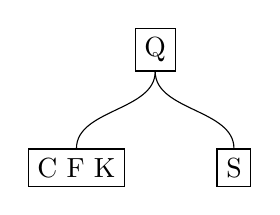
\begin{tikzpicture}[
       edge from parent path=
    {(\tikzparentnode.south) .. controls +(0,-.5) and +(0,.5)
                             .. (\tikzchildnode.north)},
    level 1/.style={sibling distance=2cm},                         
   every node/.style={draw},
   label distance=-1mm]
   
\node {Q}
    child {node {C F K}}
    child {node {S}
    };

\end{tikzpicture}
\end{center}

\begin{center}
    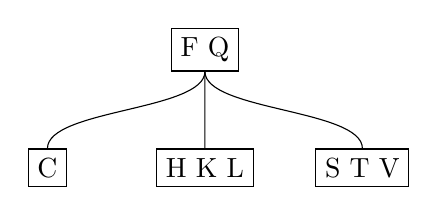
\begin{tikzpicture}[
       edge from parent path=
    {(\tikzparentnode.south) .. controls +(0,-.5) and +(0,.5)
                             .. (\tikzchildnode.north)},
    level 1/.style={sibling distance=2cm},                         
   every node/.style={draw},
   label distance=-1mm]
   
\node {F Q}
    child {node {C}}
    child {node {H K L}}
    child {node {S T V}
    };

\end{tikzpicture}
\end{center}

\begin{center}
    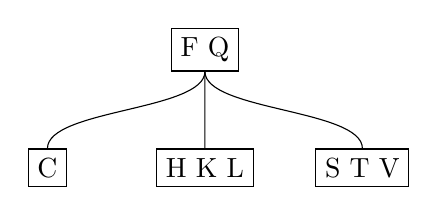
\begin{tikzpicture}[
       edge from parent path=
    {(\tikzparentnode.south) .. controls +(0,-.5) and +(0,.5)
                             .. (\tikzchildnode.north)},
    level 1/.style={sibling distance=2cm},                         
   every node/.style={draw},
   label distance=-1mm]
   
\node {F Q}
    child {node {C}}
    child {node {H K L}}
    child {node {S T V}
    };

\end{tikzpicture}
\end{center}

\begin{center}
    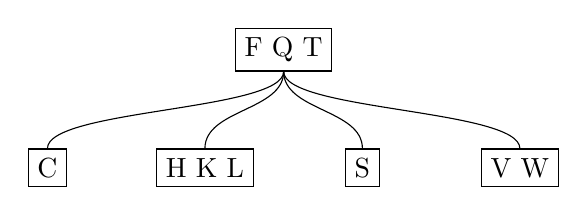
\begin{tikzpicture}[
       edge from parent path=
    {(\tikzparentnode.south) .. controls +(0,-.5) and +(0,.5)
                             .. (\tikzchildnode.north)},
    level 1/.style={sibling distance=2cm}, 
   every node/.style={draw},
   label distance=-1mm]
   
\node {F Q T}
    child {node {C}}
    child {node {H K L}}
    child {node {S}}
    child {node {V W}
    };

\end{tikzpicture}
\end{center}

\begin{center}
    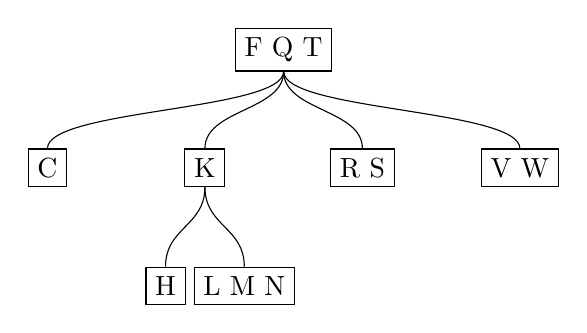
\begin{tikzpicture}[
       edge from parent path=
    {(\tikzparentnode.south) .. controls +(0,-.5) and +(0,.5)
                             .. (\tikzchildnode.north)},
    level 1/.style={sibling distance=2cm},   
    level 2/.style={sibling distance=1cm},
   every node/.style={draw},
   label distance=-1mm]
   
\node {F Q T}
    child {node {C}}
    child {node {K}
        child {node {H}}
        child {node {L M N}}
    }
    child {node {R S}}
    child {node {V W}
    };

\end{tikzpicture}
\end{center}

\begin{center}
    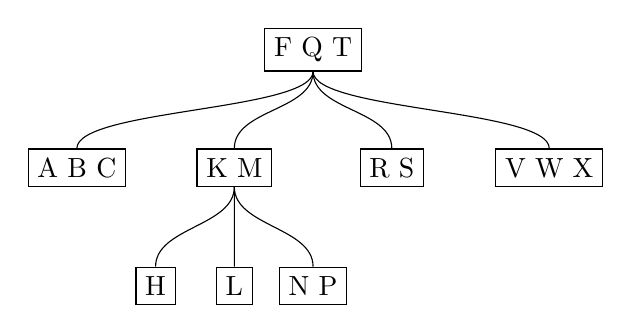
\begin{tikzpicture}[
       edge from parent path=
    {(\tikzparentnode.south) .. controls +(0,-.5) and +(0,.5)
                             .. (\tikzchildnode.north)},
    level 1/.style={sibling distance=2cm},   
    level 2/.style={sibling distance=1cm},                      
   every node/.style={draw},
   label distance=-1mm]
   
\node {F Q T}
    child {node {A B C}}
    child {node {K M}
        child {node {H}}
        child {node {L}}
        child {node {N P}}
    }
    child {node {R S}}
    child {node {V W X}
    };

\end{tikzpicture}
\end{center}

\begin{center}
    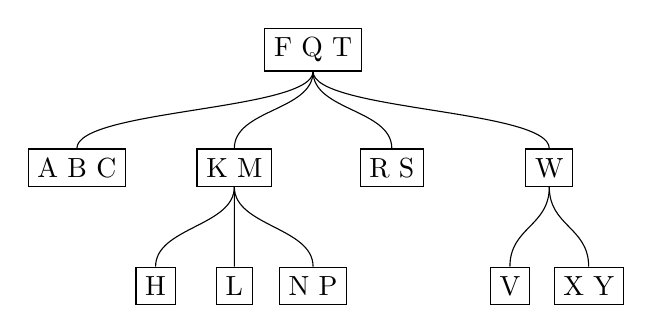
\begin{tikzpicture}[
       edge from parent path=
    {(\tikzparentnode.south) .. controls +(0,-.5) and +(0,.5)
                             .. (\tikzchildnode.north)},
    level 1/.style={sibling distance=2cm},   
    level 2/.style={sibling distance=1cm},                      
   every node/.style={draw},
   label distance=-1mm]
   
\node {F Q T}
    child {node {A B C}}
    child {node {K M}
        child {node {H}}
        child {node {L}}
        child {node {N P}}
    }
    child {node {R S}}
    child {node {W}
        child{node {V}}
        child{node {X Y}}
    };

\end{tikzpicture}
\end{center}

\begin{center}
    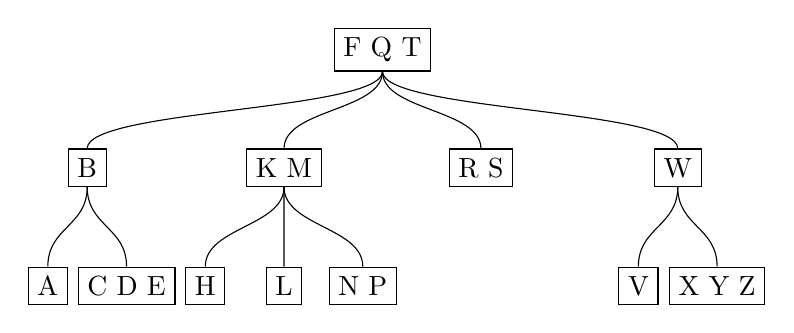
\begin{tikzpicture}[
       edge from parent path=
    {(\tikzparentnode.south) .. controls +(0,-.5) and +(0,.5)
                             .. (\tikzchildnode.north)},
    level 1/.style={sibling distance=2.5cm},   
    level 2/.style={sibling distance=1cm},                      
   every node/.style={draw},
   label distance=-1mm]
   
\node {F Q T}
    child {node {B}
        child {node {A}}
        child {node {C D E}}
    }
    child {node {K M}
        child {node {H}}
        child {node {L}}
        child {node {N P}}
    }
    child {node {R S}}
    child {node {W}
        child{node {V}}
        child{node {X Y Z}}
    };

\end{tikzpicture}
\end{center}